\documentclass[a4paper,12pt]{article}
\setlength{\headheight}{68.803pt}
\addtolength{\topmargin}{-56.803pt}

\usepackage[utf8]{inputenc}
\usepackage[T1]{fontenc}
\usepackage{lmodern}
\usepackage[nopatch=footnote]{microtype}
\usepackage{fvextra}
\DefineVerbatimEnvironment{Verbatim}{Verbatim}{
  breaklines=true,
  breakanywhere=true,
  frame=single,
  fontsize=\small
}

% margin settings
\usepackage[
  left=1in,
  right=1in,
  top=3cm,
  bottom=1in
]{geometry}

\usepackage[
    colorlinks=true,
    linkcolor=black,
    urlcolor=blue,
    citecolor=blue,
    pdfborder={0 0 0},
    pdfauthor={Massimo Mantineo},
    pdftitle={Software Defined Networking - Mininet},
    pdfsubject={Laboratorio di Reti e Sistemi Distribuiti: HANDS-ON 7},
]{hyperref}

\usepackage{graphicx}
\graphicspath{{../../assets/}{../../assets/ho1/}{../../assets/ho2/}{../../assets/ho3/}{../../assets/ho4/}{../../assets/ho5/}{../../assets/ho6/}{../../assets/ho7/}{../../assets/ho8/}{../../assets/ho10/}}
\usepackage{tikz}
\usetikzlibrary{positioning, arrows.meta}
\usepackage{listings}
\usepackage{xcolor}
\usepackage{amsmath, amssymb}
\usepackage{fancyhdr}
\usepackage{setspace}
\usepackage{pgfplots}
\pgfplotsset{compat=1.17}
\usepackage{booktabs}
\usepackage[skins, listings]{tcolorbox}
\usepackage{float}

\newtcblisting{terminal}[1][]{
    listing only,
    colback=black!85!white,
    colframe=black!70!white,
    colupper=green!80!white,
    coltitle=white,
    title=#1,
    fonttitle=\bfseries\sffamily,
    listing options={
        language={},
        basicstyle=\ttfamily\small\color{green!80!white},
        backgroundcolor={},
        frame=none,
        breaklines=true,
        showstringspaces=false,
        numbers=none
    },
    enhanced,
    drop shadow,
    arc=3mm
}

\newtcblisting{pythoncode}[1][]{
    listing only,
    colback=blue!3!white,
    colframe=blue!70!black,
    title=#1,
    fonttitle=\bfseries\sffamily,
    listing options={
        language=Python,
        basicstyle=\ttfamily\small,
        numbers=left,
        numberstyle=\tiny,
        stepnumber=1,
        numbersep=5pt,
        backgroundcolor=\color{white},
        showspaces=false,
        showstringspaces=false,
        showtabs=false,
        frame=none,
        tabsize=4,
        breaklines=true,
        breakatwhitespace=true,
        keywordstyle=\color{blue}\bfseries,
        commentstyle=\color{green!50!black},
        stringstyle=\color{red},
    },
    enhanced,
    drop shadow,
    arc=3mm
}

\setlength{\footskip}{50pt}

% Header and Footer
\pagestyle{fancy}
\fancyhf{}

\fancyhead[L]{%
  \parbox[b]{0.45\textwidth}{%
    \small
    Student Name: Massimo Mantineo\\
    Student ID: 541924
    \vspace{20pt}
  }%
}
\fancyhead[C]{%
  \parbox[b]{0.2\textwidth}{%
    \centering
    \normalsize \bfseries
    LabReSiD25\\
    Hands-On 7
    \vspace{20pt}
  }%
}
\fancyhead[R]{%
  \parbox[b]{0.35\textwidth}{%
    \flushright
    \includegraphics[width=3.5cm]{\detokenize{logo_unime_orizontale.png}}
    \vspace{15pt}
  }%
}

\renewcommand{\contentsname}{Indice}

\title{\vspace{-2cm}Report: Software Defined Networking e Mininet\\
\large (Hands-On 7)}
\author{Massimo Mantineo \\ Matricola: 541924}
\date{MESSINA, A.A. 2024/2025}

\begin{document}

% Cover page
\begin{titlepage}
    \thispagestyle{empty}
    \centering
    \vspace*{1cm}
    \includegraphics[width=6cm]{\detokenize{logo_unime_orizontale.png}}\par\vspace{1cm}
    \vspace{2cm}
    {\Large \textbf{Università degli Studi di Messina}\par}
    {\large Dipartimento MIFT - Corso di Laurea Triennale in Informatica (L-31)\par}
    \vspace*{1cm}
    {\large Laboratorio di Reti e Sistemi Distribuiti\par}
    \vspace{1cm}
    {\Large \textbf{HANDS-ON 7:}\\
    Software Defined Networking con Mininet\par}
    \vspace{2cm}
    {\large Massimo Mantineo \par}
    {\large Matricola: 541924 \par}
    \vfill
    {\large Messina, A.A. 2024/2025 \par}
\end{titlepage}

\clearpage
\pagestyle{fancy}
\tableofcontents
\newpage

\section{Problem Statement}
L'Hands-On 7 introduce il paradigma del **Software Defined Networking (SDN)** tramite l'emulatore \textbf{Mininet}. L'obiettivo dell'esercitazione è duplice: da un lato, comprendere la virtualizzazione delle risorse di rete tramite i Network Namespaces di Linux; dall'altro, progettare topologie personalizzate in Python capaci di emulare scenari reali. Il sistema deve permettere la configurazione di un router software per l'instradamento tra subnet e l'applicazione di vincoli fisici (\textit{bandwidth} e \textit{delay}) sui link virtuali per testare la robustezza dei protocolli in condizioni non ideali.

\section{Stato dell'Arte}
Il paradigma SDN rivoluziona le reti tradizionali separando il piano di controllo dal piano dei dati.

\begin{figure}[H]
    \centering
    \begin{tikzpicture}[
        node distance=1.2cm,
        plane/.style={rectangle, draw=black!60, fill=gray!5, thick, minimum width=9cm, minimum height=2.5cm, dashed},
        box/.style={rectangle, draw=purple!70, fill=purple!5, thick, minimum width=3.5cm, minimum height=1cm, align=center, font=\small\sffamily\bfseries},
        switch/.style={circle, draw=blue!70, fill=blue!5, thick, minimum size=1.2cm, font=\tiny\sffamily},
        arrow/.style={-Stealth, thick, purple!70}
    ]
        % Control Plane
        \node[plane] (control) {};
        \node[above=0.1cm of control.north, purple!70, font=\bfseries] {CONTROL PLANE (Intelligence)};
        \node[box] (controller) at (0,0) {SDN Controller\\(Mininet API / Python)};

        % Data Plane
        \node[plane, below=2cm of control] (data) {};
        \node[above=0.1cm of data.north, blue!70, font=\bfseries] {DATA PLANE (Forwarding)};
        \node[switch] (sw1) at (-2,-2.5) {vRouter};
        \node[switch] (sw2) at (2,-2.5) {vSwitch};
        
        \node[rectangle, draw=green!60, fill=green!5] (h1) at (-3.5,-3.5) {Host 1};
        \node[rectangle, draw=green!60, fill=green!5] (h2) at (3.5,-3.5) {Host 2};

        % Connections
        \draw[arrow] (controller) -- node[right, font=\tiny, color=black] {Southbound API (OpenFlow)} (0,-1.5);
        \draw[thick, blue!50] (h1) -- (sw1);
        \draw[thick, blue!50] (sw1) -- (sw2);
        \draw[thick, blue!50] (sw2) -- (h2);
        
        \node[below=0.2cm of data, font=\itshape\small] {Virtual Topology (Linux Namespaces)};
    \end{tikzpicture}
    \caption{Architettura SDN: Separazione tra logica di controllo centrallizzata e piano dati virtualizzato.}
    \label{fig:sdn_architecture}
\end{figure}

\begin{itemize}
    \item \textbf{Control Plane vs Data Plane}: In una rete SDN, l'intelligenza (routing, policy) è centralizzata in un controller software, mentre gli switch si limitano a inoltrare i pacchetti seguendo le istruzioni ricevute.
    \item \textbf{Mininet}: È l'emulatore standard de-facto per la ricerca SDN. Utilizza i container leggeri del kernel Linux per creare host, switch e router su una singola macchina, garantendo un isolamento perfetto delle interfacce.
    \item \textbf{Traffic Control (TC)}: Linux fornisce il sottosistema \texttt{tc} per gestire il queuing e la limitazione del traffico. Mininet espone questa potenza tramite la classe \texttt{TCLink}, permettendo di simulare latenze geografiche e limiti di throughput.
\end{itemize}

\section{Metodologia ed Implementazione}
L'attività è stata suddivisa in tre fasi incrementali di complessità.

\subsection{Basic Networking e Interazione L2}
Inizialmente è stata testata una topologia a switch singolo (\texttt{single,2}). L'uso di \textbf{netcat} ha permesso di validare il trasporto TCP tra host isolati.
\begin{terminal}[Test Netcat]
# h1 ascolta, h2 invia payload
h1# nc -l -p 5432
h2# nc 10.0.0.1 5432 "Hello Mininet"
\end{terminal}

\subsection{Routing L3 Personalizzato}
Tramite l'API Python di Mininet, è stato implementato un \texttt{GenericRouter}. Il nodo router abilita l'instradamento globale tramite il flag del kernel \texttt{ip\_forward}:
\begin{pythoncode}[Snippet Implementazione Router]
# Abilitazione forwarding su nodo router 'r0'
r0.cmd('sysctl net.ipv4.ip\_forward=1')
# Configurazione gateway predefinito sugli host
h1.setDefaultRoute('via 10.0.1.254')
\end{pythoncode}

\subsection{Emulazione Vincoli Fisici}
È stata applicata la classe \texttt{TCLink} per simulare un link a \textbf{100 Mbps} con un ritardo di \textbf{75ms} per ogni tratta, portando l'RTT complessivo tra host distanti a circa 300ms.


\subsection{Istruzioni di Esecuzione}
Le topologie Mininet devono essere avviate come root:
\begin{terminal}[Mininet Run]
$ sudo python3 ex2\_router.py
$ sudo python3 ex3\_tc.py
\end{terminal}

\section{Risultati}
La validazione è stata effettuata tramite tool di misura (\texttt{ping}, \texttt{iperf}) e analisi dei protocolli.

\begin{figure}[H]
    \centering
    \includegraphics[width=0.8\textwidth]{\detokenize{ho7_wireshark_ex2.png}}
    \caption{Analisi traffico SDN in topologia router-based (Esercizio 2).}
    \label{fig:sdn_router}
\end{figure}

\begin{figure}[H]
    \centering
    \includegraphics[width=0.8\textwidth]{\detokenize{ho7_wireshark_ex3.png}}
    \caption{Verifica ritardi e banda con TC su link virtuale (Esercizio 3).}
    \label{fig:sdn_links}
\end{figure}

\subsection{Analisi Wireshark}
L'ispezione della cattura (Figura 7) evidenzia graficamente l'impatto dei vincoli: i tempi tra le richieste ARP e le relative risposte riflettono esattamente il delay configurato, confermando l'accuratezza della simulazione basata su \texttt{tc}.

\subsection{Benchmark Network Constraints}
La verifica dei vincoli fisici è stata effettuata tramite le utility \texttt{ping} e \texttt{iperf} integrate nella CLI di Mininet.
\begin{terminal}[Test di Connettività e Banda]
mininet> h1 ping -c 3 h2
64 bytes from 10.0.2.1: icmp\_seq=1 ttl=63 time=300 ms
64 bytes from 10.0.2.1: icmp\_seq=2 ttl=63 time=300 ms

mininet> iperf h1 h2
*** Iperf: testing TCP bandwidth between h1 and h2 
*** Results: ['94.2 Mbits/sec', '95.1 Mbits/sec']
\end{terminal}
Il tempo di RTT misurato (300ms) corrisponde esattamente alla somma dei delay dei quattro attraversamenti dei link (75ms * 4), mentre il throughput si attesta vicino al limite dei 100 Mbps configurati, dimostrando la fedeltà del modello \texttt{TCLink}.

\section{Conclusioni e Sviluppi Futuri}
L'esperienza con Mininet ha dimostrato come la virtualizzazione permetta di testare architetture di rete complesse con costi nulli. L'integrazione tra script Python e kernel Linux rende SDN uno strumento potente per la prototipazione rapida.

\noindent \textbf{Sviluppi futuri:}
\begin{itemize}
    \item \textbf{P4 Programming}: Evoluzione verso il linguaggio P4 per definire il comportamento del Data Plane in modo ancora più granulare rispetto a OpenFlow.
    \item \textbf{Network Slicing}: Implementazione di tecniche di isolamento delle risorse per creare "fette" di rete virtuali indipendenti sopra la stessa infrastruttura fisica, anticipando le architetture 5G.
\end{itemize}
to.

\end{document}
